\documentclass[12pt,a4paper]{article}

\usepackage[ngerman]{babel}
\usepackage[T1]{fontenc}
\usepackage[utf8]{inputenc}
\usepackage{csquotes}
\usepackage{amsmath,amssymb}
\usepackage{geometry}
\usepackage{setspace}
\usepackage{hyperref}
\usepackage{graphicx}
\usepackage{float}
\usepackage{tikz}
\usetikzlibrary{arrows.meta, positioning}

\geometry{margin=2.5cm}
\onehalfspacing

\title{Kapitel 4 -- Implementierung}
\author{}
\date{}

\begin{document}
\maketitle

\section{Implementierung}

\subsection{Werkzeuge und Bibliotheken}

Die Implementierung des praktischen Teils basiert auf einer modularen
Softwarearchitektur in Python. Ziel war es, ein flexibles, reproduzierbares
und erweiterbares Analysewerkzeug zu entwickeln, das sowohl synthetische als
auch reale Netzwerke verarbeiten kann. Die Auswahl der verwendeten Werkzeuge
und Bibliotheken orientiert sich an ihrer Verbreitung in der wissenschaftlichen
Praxis sowie an ihrer Eignung für die Analyse komplexer Netzwerke.

\paragraph{Programmiersprache Python}
Als Programmiersprache wird Python eingesetzt. Python bietet eine gute Balance
zwischen Ausdrucksstärke, Lesbarkeit und Verfügbarkeit wissenschaftlicher
Bibliotheken. Insbesondere für explorative Analysen, Simulationen und
datengetriebene Auswertungen ist Python im Bereich der Netzwerkanalyse weit
verbreitet. Die Implementierung legt Wert auf klare Modulgrenzen und eine
nachvollziehbare Struktur, sodass der Code auch für Dritte leicht verständlich
bleibt.

\paragraph{NetworkX}
Die zentrale Bibliothek für die Modellierung und Analyse der Netzwerke ist
NetworkX. Sie stellt grundlegende Datenstrukturen für Graphen bereit und bietet
eine Vielzahl effizient implementierter Algorithmen zur Berechnung von
Netzwerkmetriken. Dazu zählen unter anderem kürzeste Pfade, Zentralitätsmaße,
Clustering-Koeffizienten sowie Funktionen zur Bestimmung verbundener
Komponenten.\\
Im Projekt wird NetworkX sowohl für die Erzeugung synthetischer Netzwerke als
auch für die Verarbeitung realer Netze verwendet. Durch die einheitliche
Graphrepräsentation können alle Analyse- und Simulationsschritte unabhängig vom
Ursprung des Netzwerks durchgeführt werden.

\paragraph{Datenformate und Dateiverarbeitung}
Zur Speicherung realer Netzwerke wird das GraphML-Format verwendet. GraphML ist
ein XML-basiertes Austauschformat für Graphstrukturen und wird direkt von
NetworkX unterstützt. Dadurch entfällt die Notwendigkeit eigener Parser oder
Konvertierungsroutinen innerhalb der Simulation. Reale Netzwerke, wie das aus
PyPSA-Eur abgeleitete Stromnetz, können so direkt in die Analysepipeline
integriert werden.\\
Konfigurationsdateien werden im YAML-Format abgelegt. YAML ermöglicht eine
übersichtliche und hierarchische Beschreibung experimenteller Parameter und ist
auch für größere Konfigurationen gut lesbar. Die vollständige Parametrisierung
der Experimente erfolgt über diese Dateien, wodurch Änderungen an den
Versuchsbedingungen ohne Anpassung des Programmcodes möglich sind.

\paragraph{Streamlit für die grafische Benutzeroberfläche}
Zur interaktiven Exploration der Simulationsergebnisse wird Streamlit
eingesetzt. Streamlit erlaubt es, mit vergleichsweise geringem
Implementierungsaufwand eine grafische Benutzeroberfläche zu erstellen, die
direkt mit dem Python-Code verbunden ist. Die Benutzeroberfläche dient
insbesondere dazu, Parameter zu variieren, Simulationen zu starten und
Ergebnisse visuell auszuwerten.\\
Ein besonderer Fokus liegt auf der dynamischen Visualisierung der
Netzwerkstruktur während des Simulationsverlaufs. Hierbei werden Knoten und
Kanten des Netzwerks grafisch dargestellt, sodass der schrittweise Zerfall der
Netzwerkstruktur unmittelbar sichtbar wird. Diese visuelle Komponente ergänzt
die numerischen Auswertungen und erleichtert das intuitive Verständnis der
Robustheitsphänomene.

\paragraph{Weitere Hilfsbibliotheken}
Zur numerischen Verarbeitung und Auswertung der Simulationsergebnisse werden
zusätzliche Standardbibliotheken eingesetzt. NumPy dient zur effizienten
Verarbeitung numerischer Daten, während Pandas für das Speichern, Aggregieren
und Weiterverarbeiten der Simulationsergebnisse in Tabellenform verwendet wird.
Matplotlib wird zur Erstellung statischer Plots genutzt, etwa für
Robustheitskurven oder Gradverteilungen außerhalb der interaktiven Oberfläche.

\paragraph{Begründung der Werkzeugwahl}
Die Kombination der genannten Werkzeuge ermöglicht eine klare Trennung zwischen
Modellierung, Simulation, Auswertung und Visualisierung. Gleichzeitig bleibt
das Projekt leichtgewichtig und vollständig auf Open-Source-Komponenten
aufgebaut. Dies unterstützt sowohl die Reproduzierbarkeit der Ergebnisse als
auch die Nachvollziehbarkeit der Implementierung, was insbesondere im
akademischen Kontext von zentraler Bedeutung ist.


\subsection{Softwarearchitektur und Modulaufbau}

Die Software ist modular aufgebaut und folgt einer klaren Trennung zwischen
Konfiguration, Netzwerkgenerierung, Simulation, Auswertung und Visualisierung.
Ziel dieser Struktur ist es, die einzelnen Arbeitsschritte der Analyse
nachvollziehbar zu isolieren und gleichzeitig eine flexible Erweiterbarkeit zu
ermöglichen, gemäß dem Softwaredesignprinzip Seperation of Concerns (SoC). Die Architektur orientiert sich dabei nicht an klassischen
Software-Frameworks, sondern an der logischen Abfolge eines experimentellen
Workflows.

\paragraph{Gesamtstruktur des Projekts}
Das Projekt ist in mehrere Hauptverzeichnisse gegliedert. Der Quellcode
befindet sich im Verzeichnis \texttt{src/}, während Konfigurationsdateien unter
\texttt{configs/} abgelegt sind. Eingabedaten für reale Netzwerke werden in
\texttt{data/} gespeichert, wobei eine Trennung zwischen Rohdaten und
aufbereiteten Graphdateien vorgenommen wird. Simulationsergebnisse werden
strukturiert im Verzeichnis \texttt{results/} abgelegt.
Diese Trennung ermöglicht es, Konfigurationen, Daten und Code unabhängig
voneinander zu verändern. Insbesondere können neue Experimente durch das
Hinzufügen oder Anpassen von YAML-Dateien definiert werden, ohne dass
Änderungen an der Implementierung erforderlich sind.

\begin{figure}[htbp]
  \centering
  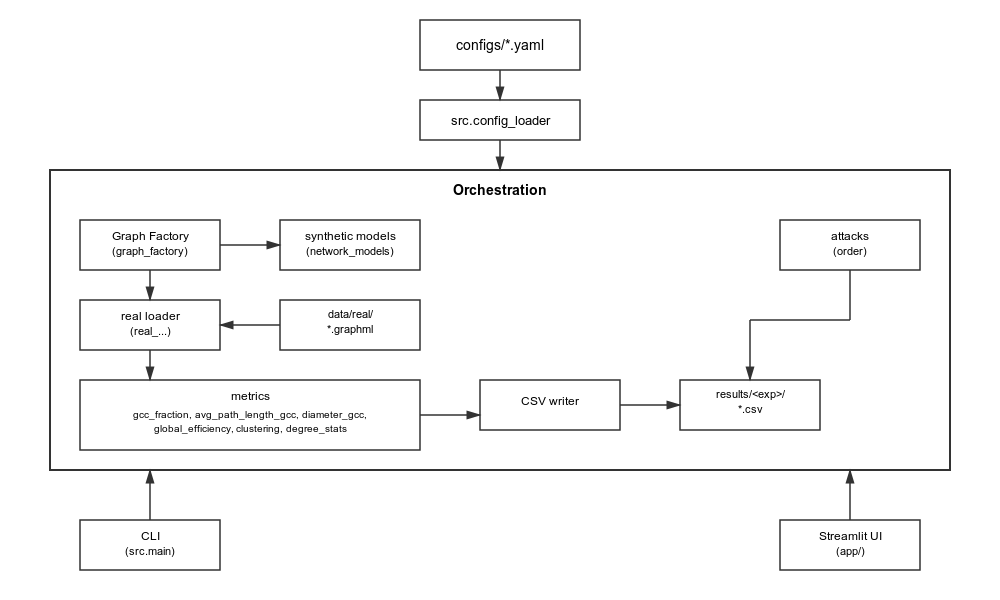
\includegraphics[width=\textwidth]{figures/architecture.png}
  \caption{Architektur des Simulationsprojekts. Die Simulation wird vollständig über
  Konfigurationsdateien gesteuert und modular in Netzwerkgenerierung,
  Angriffsszenarien, Metrikberechnung und Ergebnisverarbeitung unterteilt.}
  \label{fig:projektarchitektur}
\end{figure}


\paragraph{Konfigurations- und Steuerungsebene}
Die Konfiguration der Experimente erfolgt vollständig über YAML-Dateien. Das
Laden und Validieren dieser Konfigurationen wird durch das Modul
\texttt{src/config\_loader.py} realisiert. Dieses Modul stellt sicher, dass
alle benötigten Parameter vorhanden sind und in einer einheitlichen internen
Struktur an die weiteren Komponenten des Systems übergeben werden.\\
Die zentrale Steuerung eines Experiments erfolgt über das Modul
\texttt{src/simulation.py}. Dieses Modul koordiniert den gesamten Ablauf eines
Simulationslaufs, beginnend bei der Netzwerkgenerierung über die Anwendung der
Störungsszenarien bis hin zur Berechnung der Metriken und dem Speichern der
Ergebnisse. Dadurch fungiert \texttt{simulation.py} als verbindende Schicht
zwischen den einzelnen Funktionsmodulen.

\paragraph{Netzwerkgenerierung und Datenanbindung}
Die Erzeugung synthetischer Netzwerke ist im Modul \texttt{src/network\_models.py}
implementiert. Dort sind die verschiedenen Netzwerkmodelle (Erdős--Rényi,
Watts--Strogatz, Barabási--Albert) gekapselt, sodass sie über eine einheitliche
Schnittstelle instanziiert werden können. Für reale Netzwerke wird ein separater Ladepfad verwendet. \\
Das Modul \texttt{src/real\_network\_loader.py} übernimmt das Einlesen von GraphML-Dateien
sowie optionale Vorverarbeitungsschritte, etwa die Beschränkung auf die größte
verbundene Komponente oder die Umnummerierung der Knoten. Die Auswahl, ob ein
synthetisches oder reales Netzwerk erzeugt wird, erfolgt zentral über das Modul
\texttt{src/graph\_factory.py}, das als Abstraktionsschicht zwischen
Konfiguration und konkreter Netzwerkgenerierung dient.

\paragraph{Störungsszenarien und Angriffsauswahl}
Die Definition der Störungsszenarien ist im Modul \texttt{src/attacks.py}
umgesetzt. Dieses Modul berechnet für ein gegebenes Netzwerk die Reihenfolge,
in der Knoten im Rahmen eines bestimmten Angriffsszenarios entfernt werden
sollen. Dabei werden sowohl zufällige Ausfälle als auch gezielte Angriffe auf
Basis von Zentralitätsmaßen unterstützt.\\
Durch die Auslagerung der Angriffsauswahl in ein eigenes Modul wird eine klare
Trennung zwischen der Definition der Störung und ihrer Anwendung erreicht. Neue
Angriffsszenarien können so implementiert werden, ohne den Ablauf der
Simulation selbst verändern zu müssen.

\paragraph{Metrikberechnung und Analyse}
Die Berechnung aller strukturellen Metriken erfolgt im Modul
\texttt{src/metrics.py}. Dieses Modul enthält Funktionen zur Bestimmung der
Größe der größten verbundenen Komponente, von Clustering-Koeffizienten,
Durchmesser, Effizienz und weiteren Kenngrößen. Die Metrikfunktionen sind
bewusst unabhängig von der Simulation implementiert, sodass sie auch isoliert
auf einzelne Netzwerke angewendet werden können.\\
Die weiterführende Auswertung der Simulationsergebnisse, insbesondere die
Aggregation über mehrere Wiederholungen sowie die Berechnung der
Robustheitskennzahlen wie der Fläche unter der Robustheitskurve, erfolgt im
Modul \texttt{src/analysis.py}. Diese Trennung erleichtert eine saubere
Nachvollziehbarkeit der einzelnen Verarbeitungsschritte.

\paragraph{Visualisierung und Benutzeroberfläche}
Die grafische Benutzeroberfläche ist im Verzeichnis \texttt{app/} umgesetzt und
basiert auf Streamlit. Die Datei \texttt{streamlit\_app.py} verbindet die
Konfigurations-, Simulations- und Analysekomponenten zu einer interaktiven
Oberfläche. Neben tabellarischen und grafischen Auswertungen wird dort auch
eine dynamische Visualisierung der Netzwerkstruktur realisiert, die den
schrittweisen Zerfall des Netzwerks während der Simulation sichtbar macht.\\
Die eigentliche Logik zur dynamischen Netzvisualisierung ist im Modul \\
\texttt{src/dynamic\_visualization.py} gekapselt. Dadurch bleibt die
Benutzeroberfläche übersichtlich, während die Visualisierungslogik unabhängig
weiterentwickelt werden kann.

\paragraph{Architektonische Einordnung}
Die gewählte Architektur folgt keinem monolithischen Ansatz, sondern
orientiert sich an der logischen Trennung der experimentellen Aufgaben. Diese
Struktur unterstützt sowohl die Erweiterbarkeit des Projekts als auch dessen
Verständlichkeit. Gleichzeitig bleibt die Implementierung bewusst einfach
gehalten, um den Fokus auf die inhaltliche Analyse der Netzwerke und nicht auf
komplexe Softwarearchitektur zu legen.

\subsection{Reproduzierbarkeit und Konfigurationsmanagement}

Ein zentrales Ziel der Implementierung ist die vollständige
Reproduzierbarkeit aller durchgeführten Experimente. Da die Analyse komplexer
Netzwerke sowohl stochastische Prozesse als auch zufallsbasierte
Netzgenerierung umfasst, ist ein transparentes und konsistentes
Konfigurationsmanagement notwendig. Dieses wird im Projekt durch eine klare
Trennung von Code, Konfiguration und Ergebnisdaten realisiert.

\paragraph{Konfigurationsdateien}
Alle experimentellen Parameter werden ausschließlich über YAML-basierte
Konfigurationsdateien im Verzeichnis \texttt{configs/} definiert. Diese
Dateien enthalten sämtliche Informationen zur Beschreibung eines Experiments,
darunter die Auswahl der Netzwerkmodelle, deren Parametrisierung, die
betrachteten Störungsszenarien, die Schrittweite der Knotenentfernung sowie
die zu berechnenden Metriken.\\
Durch diese Auslagerung der Konfiguration aus dem Programmcode können neue
Experimente definiert oder bestehende Experimente variiert werden, ohne
Änderungen an der Implementierung vornehmen zu müssen. Gleichzeitig bleibt die
vollständige Beschreibung eines Experiments in einer einzelnen Datei
nachvollziehbar dokumentiert.

\paragraph{Zufallsstartwerte und deterministisches Verhalten}
Zur Kontrolle stochastischer Einflüsse werden alle zufallsbasierten Prozesse
durch explizite Zufallsstartwerte (Seeds) gesteuert. Diese betreffen sowohl
die Generierung synthetischer Netzwerke als auch die Auswahl zufälliger
Ausfallreihenfolgen bei Random-Failure-Szenarien. Die verwendeten Seeds sind
Bestandteil der jeweiligen Konfigurationsdateien.

Durch dieses Vorgehen ist sichergestellt, dass identische
Konfigurationsdateien bei mehrfacher Ausführung zu denselben Netzwerken,
Ausfallreihenfolgen und Simulationsergebnissen führen. Dies ermöglicht nicht
nur eine zuverlässige Reproduktion der Ergebnisse, sondern auch einen gezielten
Vergleich einzelner Parameteränderungen.

\paragraph{Ergebnisstruktur und Versionierung}
Die Ergebnisse der Simulationen werden automatisiert im Verzeichnis
\texttt{results/} abgelegt. Für jedes Experiment wird ein eigener Unterordner
erzeugt, der sowohl die Rohdaten der einzelnen Simulationsläufe als auch
aggregierte Auswertungen enthält. Die Dateinamen enthalten den Namen des
Experiments, sodass eine eindeutige Zuordnung zwischen Konfiguration und
Ergebnisdaten möglich ist.\\
Die Speicherung der Ergebnisse in tabellarischer Form ermöglicht eine spätere
Weiterverarbeitung, etwa für zusätzliche Analysen oder externe
Visualisierungen. In Kombination mit einer Versionsverwaltung des Quellcodes
lassen sich so auch ältere Ergebnisse eindeutig einem bestimmten Stand der
Implementierung zuordnen.

\paragraph{Nachvollziehbarkeit des Experimentablaufs}
Durch die Kombination aus konfigurationsbasierter Steuerung, deterministischer
Simulation und strukturierter Ergebnisablage ist der gesamte Experimentablauf
transparent nachvollziehbar. Jeder Schritt von der Definition der Parameter
bis zur Auswertung der Ergebnisse lässt sich rekonstruieren. Dieses Vorgehen
entspricht gängigen wissenschaftlichen Standards und stellt sicher, dass die
im Rahmen dieser Arbeit präsentierten Ergebnisse überprüfbar und
reproduzierbar sind.

\end{document}